\documentclass[a4paper, 12pt]{article}

\usepackage[utf8]{inputenc}
\usepackage{graphicx}
\graphicspath{{./Bilder/}}
\usepackage[T1]{fontenc}
\usepackage[ngerman]{babel}
\usepackage{hyperref}
\usepackage[a4paper, left=2.5cm, right=2.5cm, top=2.5cm]{geometry}
\renewcommand{\baselinestretch}{1.5}
\usepackage{cite}
\usepackage{bibgerm}
\usepackage{longtable}

\author{Tobias Sigmann}
\title{Seminararbeit: LoRaWAN}
\date{\today}

\begin{document}
    \maketitle
    \newpage
    \tableofcontents
    \newpage

    \section{Einführung}
        Warum noch eine weiteres Funknetz? 
        Reichen die bestehenden Funknetzt nicht aus?

        Heutige freie Funknetze sind GSM, Wi-Fi, Bluetooth, usw.
        
        In jedem Funknetz sind drei Parameter wichtig: Bandbreite/Übertragungsrate, Energiebedarf und Reichweite.
        Wi-Fi hat eine hohe Bandbreite, hoher Energiebedarf und eine begrenzte Reichweite. 
        GSM hat eine höhere Bandbreite, einen hohen Energiebedarf und mittlere Reichweite.
        Bluetooth hat geringe Bandbreite, eine niedringen Energiebedarf und eine niedrige Reichweite.
        
        Für sehr hohe Reichweiten und sehr niedringen Energiebedarf gab es bisher noch keine Lösung.
        Hier setzen nun Low-­Power-Wide-Area-Netzwerk-Technologien
        (LPWAN) wie LoRa, Sigfox und NarrowBand-IoT (NB-IoT) an. Diese Netzwerke sind für IoT,
        Smart-City-Applikationen und andere LPWAN-Anwendungen geeignet.
        Beispiele sind smarte Mülleimer, Straßenlaternen, Parkplätze aber auch privat für SmartHomes geeignet.
        Der Vorteil einer sehr hohe Reichweiten (bis zu 20km) und sehr niedringen Energiebedarf (Batterielaufzeit
        bis zu mehreren Jahren) hat den Nachteil einer sehr gerigen Bandbreite (zwischen 0.3 und 50 kbps). 


        \begin{figure}[h]
            \centering
            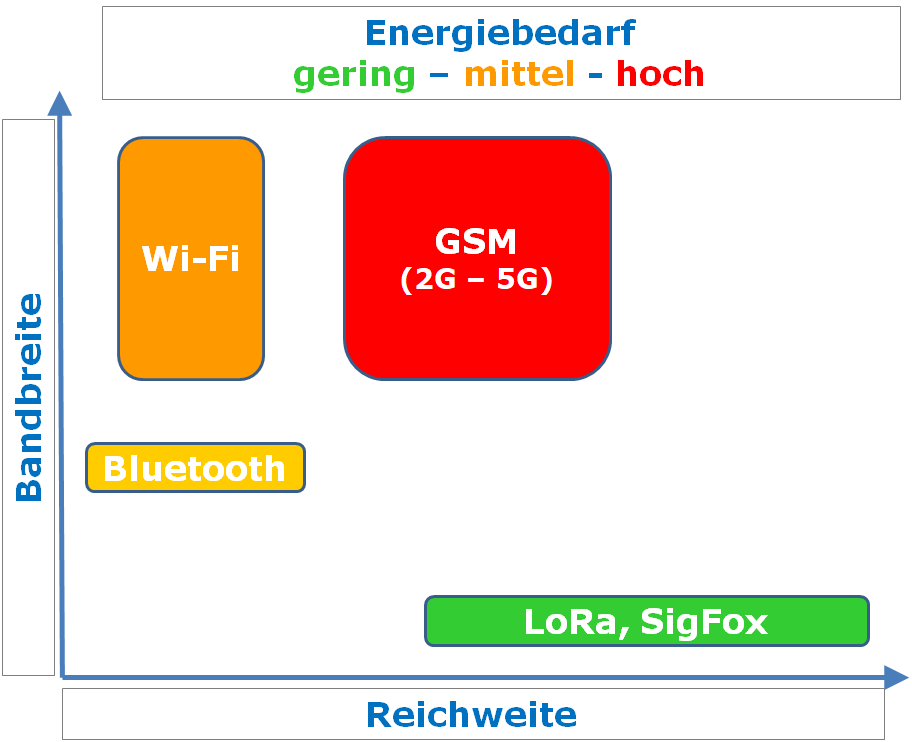
\includegraphics[width=13cm, height=7cm]{Einfuehrung}
            \caption{Funknetzvergleich}
        \end{figure}

        Im folgenen wird der Aufbau und die Funktion von LoRaWAN 1.1 beschreiben.\newline
        LoRaWAN steht für ``Long Range Wide Area Network''. \cite{WhatIsLoRa}

        
        
    \section{Aufbau eines LoRa-Netzwerk}
        LoRa ist ideal für IoT-Geräte, da per einfachem Netzwerkaufbau Datenaustausch mit dem Internet möglicht ist.
        Um die von den End-Geräten gesendeten LoRa-Pakete auf IP/TCP Pakete umzusetzen wird ein Gateway als Schnittstelle
        benötigt, um die LoRa-Pakete in TCP/IP Pakete umzuwandeln und umgekehrt.
        Das Gateway implementiert aber keinerlei Logik. Hierzu ist ein Netzwerkserver zuständig der über die 
        Gateways das Netzwerk kontrolliert und steuert. Gleichzeitig stellt er die Verbindung zu einem 
        Applikationsserver her, indem er die Daten weiterleitet.

        Der Applikationsserver ist zuständig die gesendeten Nachrichten zu verarbeiten und sendet Daten an die 
        Endgeräte.

        Diese Architektur wurde gewählt um geringen Energieverbrauch zu ermöglichen bei gleichzeitiger 
        hoher Endgeräteanzahl, hoher Siganlqualität und entsprechnder Netzwerksicherheit. \cite[S. 8 ff.]{WhatIsLoRa}
        
        \subsection{Gateway}
            Die LoRa-Endgeräte werden sternförmig an die Gateways angeschlossen und stellen ein Teilnetz dar. 
            Jedes Endgeräten kommuniziert direkt mit dem Gateway. Diese Art der Kommunikation wird  
            ``Single-Hop-Connection'' genannt, da die gesendeten Daten ohne Umwege an das Gateway gesendet werden. 
            Jedes Gateway ist mit mindestens einem Netzwerkserver verbunden.
        
            Ein Endgerät kann gleichzeitig an mehreren Gateways senden. Der Netzwerkserver überprüft die Pakete 
            auf Duplikate und stellt sicher dass jedes Paket nur einmal an die Applikationsserver gesendet werden.
            Ein weiterer Vorteil ist das keine Endgeräteübergabe zwischen den Gateways bei Standortwechsel nötig sind.
            Da die Gateways mit allen in der Reichweite befindlichen Endgeräten kommunizieren müssen, wurde 
            auf Einzelkommunikation verzichtet und auf Parallelkommunikation gesetzt. 
            Dazu werden adaptive Datenraten und Mehrkanal-Multi-Modem-Transceiver verwendet.
        
            Durch die genannt Eigenschaften der Gateways wird eine gute Skalierbarkeit erzielt. Dadurch können neue 
            Gateways die Anzahl der Endgeräte um das sech bis acht-fach erhöhen. vgl. \cite[S.10]{WhatIsLoRa}
        \subsection{Netzwerkserver}
            Der Netzwerkserver ist das ``Herzstück‘‘ eines jeden LoRa-Netzwerkes. Er kann mit mehreren Gateways und 
            mehreren Applikationsserver verbunden sein. 

            Die wichtigste Aufgabe des Netzwerksserver ist die Steuerung des LoRa-Netzwerks. Der Server 
            verwaltet jedes Endgerät separat, indem es mit ihm den zu verwendenden Funkkanal aushandelt und die Datenrate
             kontrolliert wenn ADR (Adaptiv Data Rate) aktiv ist. Außerdem steuert er den Netzwerkbeitritt der 
             Endgeräte.

            Weiterhin überprüft er die empfangen Pakete auf ihre Korrektheit und Integrität. Wie auch schon erwähnt 
            filtert er Duplikate.
            Dabei ermittelt er auch das Gateway mit dem besten Empfang zum jeweiligen Endgeräten und nutzt 
            dieses dann um Daten an das Endgerät zu senden.

            Es ist nicht immer möglich Daten direkt zu senden, da die Endgeräte nicht immer empfangsbereit sind. Um 
            die Applikationsserver zu entlasten, puffert der Netzwerkserver die Daten und sendet diese zum nächst 
            möglichen Zeitpunkt.

            Eine weitere sehr wichtige Ausgabe ist es eine Schnittstelle für den Applikationsserver bereitzustellen 
            um eine 
            einfache und schnelle Kommunikation zu ermöglichen.
        \subsection{Join-Server}
            Ein Join-Server wird benötigt um den Beitritt mittels OTAA zu ermöglichen. Mehr zu OTAA kann in dem 
            Kappitel \ref{sec:OTAA} \nameref{sec:OTAA} gelesen werden. Wenn ein Endgerät dem Netzwerk beitreten möchte, leitet 
            der Netzwerkserver die Anfragen an den Join-Server weiter. Dieser führt dann die nötige Beitrittschritte 
            aus, wie z.B. Ableiten von Schlüsseln oder Senden der nötigen Einstellungen. Dafür ist der NwkKey und 
            der AppKey notwendig, da diese zum Verschlüsseln der Nachrichten benötigt werden. 
            Aus Sicherheitsgründen dürfen diese Schlüssel nie über das LoRa-Netz übertragen werden, sondern müssen
            bei der Programmierung des Endgerätes vorgegeben werden. \cite[S. 9 f.]{LoRaBack}

            Der Join-Server kann mit mehreren Netzwerkservern verbunden werden und jeder Netzwerkserver kann mehrere 
            Join-Server haben.
        \subsection{End-Gerät}\label{sec:endgerät}
            Endgeräte sind Geräte die Informationen mittels LoRa empfangen oder senden. Jedes Endgerät ist mit einem 
            bestimmten Applikationsserver verbunden.

            Jedes Endgerät muss zur korrekten Funktion mehrere wichtige Informationen haben.
            \begin{itemize}
                \item DevEUI: Globale Endgeräte\_ID, die eindeutig für jedes Endgerät definiert ist. Vergleichbar 
                mit der MAC-Adresse eines TCP/IP Gerätes.
                \item JoinEUI: Globale Adresse des Join-Servers, an den die Join-Anfrage gehen soll. Wird nur für OTAA Geräte
                benötigt.
                \item NwkKey und AppKey: Werden verwendet um spätere Schlüssel abzuleiten und die Kommunikation während
                der Beitrittprozedur in ein Netzwerk abzusichern. Dafür müssen sie sowohl dem Join-Server als auch dem
                Endgerät bekannt sein.
            \end{itemize}
            \cite[S.47 ff.]{LoRaSpec}

    \section{LoRaWAN Funktionsweise}
        Im folgenden Kapitel wird näher auf die Funktionsweise von LoRaWAN eingegangen. Speziell liegt der Fokus auf
        dem Netzwerkbeitritt, das verwendete Protokoll und wie die Daten physikalisch übertragen werden.
        \subsection{Schichtenmodell}
            \begin{figure}
                \includegraphics[width=\textwidth]{LoRaLayer}
                \caption{LoRaStack \cite[S.7]{WhatIsLoRa}}
            \end{figure}
            Das Schichtenmodell lässt sich in zwei Teile unterteilen. Der LoRa-Part ist der unterste und kümmert sich 
            um die physikalische Übertragung der Pakte. Der LoRaWAN-Part ist für die Steuerung des 
            Netzwerkes, Definition der LoRaWAN-Klassen und das Überprüfen / Verschlüsseln der Daten zuständig.

            Die unterste Schicht des LoRa-Parts ist für die Anwendung der richtigen Frequenzen zuständig. In Europa 
            muss das freiverfügbare ISM-Band 868 verwendet werden, in den Vereinigten Staaten das Band 915 und 
            in Asien das Band 430 .\cite[S.7]{WhatIsLoRa}

            Die darüber liegende Schicht nennt man LoRa-Modulation. Sie wandelt die binären Pakete in 
            LoRa-Signale um, so dass der Empfänger diese korrekt und effizient empfangen und wiederherstellen 
            kann. Mehre dazu im Kapitel  \ref{sec:Modulation} \nameref{sec:Modulation}

            Über LoRa-Modulation liegt die erste LoRaWAN-Schicht die LoRa-MAC genannt wird. MAC steht für ``Media Access 
            Protokoll''. Dieses Protokoll wird zur Steuerung des LoRa-Netz verwendet. Diese Schicht ist außerdem für 
            die Implementierung der einzelnen Endgeräteklassen 
            und für das Übertragen der Steuerungskommandos zuständig. Mehr zu den Endgeräteklassen kann im Kapitel 
            \ref{sec:klassen} \nameref{sec:klassen} und im Kapitel \ref{sec:protokoll} \nameref{sec:protokoll} gelesen werden.

            Die oberste Schicht nennt sich Applikationsschicht und verpackt, verschlüsselt und authentifiziert 
            die Nutzdaten einer Nachricht.
        \subsection{Netzwerkbeitritt}
            Endgeräte sind immer einem bestimmten Netzwerk zugeordnet. Es gibt zwei Wege um ein neues Endgeräte zu einem 
            bestehenden Netzwerk hinzuzufügen.
            \subsubsection{OTAA} \label{sec:OTAA}
                Die sicherste aber auch aufwendigste Methode heißt 
                OTAA ``Over-the-Air Activation''. Hierbei muss bei jedem Netzwerkbeitritt die Join-Prozedur ausgeführt
                werden. Dafür müssen folgende 4 Konstanten im Programm vorhanden sein: DevEUI, 
                JionEUI, NwkKey und AppKey.

                Näheres zu den Konstanten kann im Kapitel \ref{sec:endgerät} \nameref{sec:endgerät} nachgelesen werden.

                Der NWKSKEY ist für die Verschlüsslung der Datenpakete bis zu Gateway zuständig. Dieser Key wird 
                vom Netzwerkserver erzeugt und muss manuell in den Code eingetragen werden.\cite[S.3]{LoRaSecur}
            
                Der letzte Wert heißt APPSKEY und sichert die Kommunikation vom Endgerät zu dem Applikationsserver ab. 
                Der Schlüssel wird genau wie der NWKSKEY vom Netzwerkserver erzeugt und verwaltet.\cite[S.3]{LoRaSecur}

                Als erstes muss das End-Gerät eine Join- oder Rejoin-Nachricht an das Gateway senden. Die Nachricht besteht aus der 
                JoinEUI, dem DevEUI und einer DevNonce. Mit der DevNonce sollen Replayattack verhindert werden. Die
                Nonce startet beim ersten Join-Request mit 0 und wird bei jedem Join-Request um eins erhöht. 
                Die Nonce muss im einem nichtflüchtigen Speicher gespeichert werde, um die Werte unter allen Bedingungen 
                zu sichern. Ansonsten wäre ein manueller Reset des Zählers im Netzwerkserver erforderlich.
                Sendet ein Endgerät einen Join-Request mit zu kleinem DevNonce, wird die Nachricht ignoriert und es 
                ist nicht möglich dem Netzwerk 
                beizutreten.

                Das Gateway antwortet mit einer Accept-Nachricht, besteht aus einer JoinNonce, einem NetzwerkID Net\_ID, einer Geräteadresse DevAddr,
                einem Einstellungsfeld DLSettings , einer Zeitangabe wie lange zukünftig auf eine Antwort nach dem
                Senden gewartet werden muss (hier RxDelay) und einer optionalen Netzwerkparameterliste CFList.

                Die JoinNonce wird verwendet um Replayatacken zu verhindern und muss größer als die zuletzt 
                gesendete sein. Ansonsten wird die Nachricht vom Endgerät ignoriert. Außerdem wird die Nonce benutzt 
                um Schlüssel wie 
                AppSKey herzuleiten. Für jedes Endgerät wird eine eigene JoinNonce geführt, sie darf sich nicht 
                wiederholen. Jedes Endgerät merkt sich die letzte JoinNonce und tritt auch nur bei, wenn diese größer 
                ist als die letzte.

                Die Join-Accept Nachricht wird vom Endgerät nach JOIN\_ACCEPT\_DELAY1 oder JOIN\_ACCEPT\_DELAY2 nach 
                dem Senden des Request erwartet. Wird die Join-Accept Nachricht zu einem andern Zeitpunkt gesendet,
                wird diese nicht empfangen, da das Endgerät nicht empfangsbereit ist.

                Mehr Informationen zu den Ableitungen der Schlüssel finden Sie in dem Kapitel \ref{sec:Sicherheit} \nameref{sec:Sicherheit}.

            \subsubsection{ABP}
                Die einfachste Art des Beitritts heißt ABP was für ``Activation by Personalization'' steht. 
                Hierbei muss lediglich vor Inbetriebnahme des 
                Endgerätes fünf Konstanten definiert werden. 

                Als erstes wird die DevAdr(Geräteadresse) angegeben. Diese Adresse existiert nur einmal im 
                Netzwerk und wird für die Indentifizierung des Endgeräts verwendet. Die Adresse wird vom Netzwerkserver 
                erzeugt und muss im Programmcode eingetragen sein.

                Die anderen vier Werte sind die verwendeten Schlüssel zur Kommunikationsverschlüsselung:  
                FNwkSIntKey, SNwkSIntKey, NwkSEncKey und AppSKey. Damit kann die Join-Prozdeur 
                übersprungen werden. Allerdings werden immer dieselben Schlüssel verwendet, was zu einem 
                Sicherheitsproblem werden kann.

                Nach Beitritt muss das ResetInd MAC-Kommando im FOpt Feld gesendet werden. Dieses Kommando 
                teilt dem Netzwerkserver mit, dass das Endgerät online ist und die Standardübertragungsart, 
                -frequenz und -kanal verwendet werden. Weiter Erläuterungen folgen im nächsten Unterkapitel.

                Das Netzwerk muss  mit einem ResetConf-Kommando antworten. In diesem teilt es dem Endgerät die
                unterstützten LoRa-Versionen mit. Danach kann die Kommunikation beginnen.
        \subsection{Protokoll} \label{sec:protokoll}
            Das LoRaWAN-Protokoll ist optimiert für batteriebetrieben Endgeräte für drahtlos Kommunikation. 
            Um energieeffizent zu sein setzt LoRa hauptsächlich auf zwei Punkte: die Modulationstechnik und  
            Adaptive Datenrate (ADR). Auch die 
            ``One-Hop'' Architektur trägt zur Energieeffizenz bei. Die Modulationsart wird in Kapittel 
            \ref{sec:Modulation} \nameref{sec:Modulation} beschrieben. \cite[S,1 f]{LoRaClasses}


            Damit der Netzwerkserver das LoRa-Netz steuern kann, werden Mac-Kommandos eingesetzt. Mit diesen 
            Kommandos tritt man dem Netzwerk bei, kommuniziert mit den Endgeräten und steuert
            Frequenzen, Kanäle und vieles mehr.
            Da die Kommandos nur für den Netzwerkserver und die Endgeräte von Bedeutung sind, werden diese nicht an 
            den Applikationsserver gesendet, sondern vom Netzwerkserver herausgefiltert. Im folgenden wird näher auf 
            die MAC-Kommandos und die Paketstruktur eingegangen.
            Ein Uplink ist ein Paket das vom Endgerät, das bildlich gesprochen ``unter‘‘ dem Gateway sitzt, an das 
            Gateway gesendet wird. Ein Downlink ist dem entsprechend ein Paket, das vom Gateway an das Endgerät gesendet 
            wird.
            \subsubsection{MAC-Kommandos}
                MAC-Kommandos werden ausschließlich für die Steuerung und Pflege des Netzwerkes verwendet. MAC steht 
                für ``Medium Access Control‘‘. Da der Netzwerkserver das Netzwerk steuert, werden diese Kommandos nur 
                zwischen dem Netzwerkserver und dem Endgerät verwedet.

                MAC-Kommandos werden mittels eines ``Command Indentifier‘‘ (CID) gesendet. Das ist eine 8 Bit Zahl die 
                das MAC-Kommando repräsentiert. Nach dem CID folgen mögliche Variablen die dem Kommando mitgegeben 
                werden. Die Anzahl und Länge der Variablen ist nicht beschränkt.
                
                Die MAC-Kommandos müssen zwingend ausgeführt werden. Die Nachrichten werden in derselben Reihenfolge 
                wie sie angekommen bestätigt oder beantwortet. Somit weiß der Netzwerkserver welche Kommandos 
                bereits ausgeführt wurden. Alle Kommandos die in einem Frame gesendet wurden, müssen auch in einem Frame  
                bestätigt/beantwortet werden. Zur Speicherung der Reihenfolge wird ein Puffer für die 
                MAC-Kommando-Antworten verwendet. Dieser Puffer wird beim nächsten Uplink mit gesendet. 
                Sollte der Puffer zu klein sein, werden keine weiteren Antworten eingetragen. 
                Deshalb muss der Netzwerkserver vorher die maximale Antwortgröße errechnen und die 
                MAC-Kommandos dementsprechend in Frames aufteilen.\cite[S.29 ff.]{LoRaSpec}

                Im Folgenden ist eine Liste aller MAC-Kommandos angegeben:
           
                    
                \begin{longtable}{c |c | p{10.5cm} c}
                    CID & Kommandoname & Funktion \\
                    \hline
                    0x01 & ResetInd & Wird bei dem Beitritt mittels ABP vom Endgerät gesendet. Informiert das Netzwerk über den Beitritt. \\
                    0x01 & ResetConf & Wird vom Gateway gesendet und bestätigt das ResetInd-Kommando. \\
                    0x02 & LinkCheckReq & Wird vom Endgerät verwendet um die Verbindung zum Netzwerk zu überprüfen. \\
                    0x02 & LinkCheckAns & Bestätigt das vom Endgerät gesendete LinkCheckReq-Kommando \\
                    0x03 & LinkADRReq & Wird zu Steuerung der Endgeräte im ADR-Modus verwendet \\
                    0x04 & DutyCycleReq & Das Gateway teilt dem Endgerät mit wie oft die Verbindung getestet werden soll \\
                    0x04 & DutyCycleAns & Das Endgerät bestätigt den neuen Testzyklus \\
                    0x05 & RXParamSetupReq & ... \\
                    0x05 & RXParamSetupAns & ... \\
                    0x06 & DevStatusReq & ... \\
                    0x06 & DevStatusAns & ... \\
                    0x07 & NewChannelReq & ... \\
                    0x07 & NewChannelAns & ... \\
                    0x08 & RXTimingSetupReq & ... \\
                    0x08 & RXTimingSetupAns & ... \\
                    0x09 & TxParamSetupReq & ... \\
                    0x09 & TxParamSetupAns & ... \\
                    0x0A & DlChannelReq & ... \\
                    0x0A & DlChannelAns & ... \\
                    0x0B & RekeyInd & ... \\
                    0x0B & RekeyConf & ... \\
                    0x0C & ADRParamSetupReq & ... \\
                    0x0C & ADRParamSetupAns & ... \\
                    0x0D & DeviceTimeReq & ... \\
                    0x0D & DeviceTimeAns & ... \\
                    0x0E & ForceRejoinReq & ... \\
                    0x0F & RejoinParamSetupReq & ... \\
                    0x0F & RejoinParamSetupAns & ... \\
                    0x10 & PingSlotInfoReq & ... \\
                    0x10 & PingSlotInfoAns & ... \\
                    0x11 & PingSlotChannelReq & ... \\
                    0x11 & PingSlotChannelAns & ... \\
                    0x12 & BeaconTimingReq & ... \\
                    0x12 & BeaconTimingAns & ... \\
                    0x13 & BeaconFreqReq & ... \\
                    0x13 & BeaconFreqAns & ... \\
                    0x20 & DeviceModeInd & ... \\
                    0x20 & DeviceModeConf & ... \\
                    0x80-0xFF & Proprietary & ... \\
                    
                    
                \end{longtable}
                


            \subsubsection{LoRa-Paketstruktur}
                Die Paketstruktur kommt wie beim ISO/OSI Schichtenmodel durch das ``durchlaufen‘‘ des Stacks zustande. 
                Die Paketstruktur wird hier Top-Down betrachtet. Als erstes werden die Felder
                der Modulationsschicht betrachtet.

                Jedes Pakete besteht grundlegend aus zwei Felder: Präambel und PHYPayload. Falls es sich um einen 
                Uplink-Paket handelt wird noch ein CRC Code hinzugefügt, also Preamble, PHYPayload, CRC. 
                In diesem Fall spricht man von einem impliziten Paket oder vom implizitem Modus. Impliziter Modus bedeute, 
                dass es kein Payload Header gibt. Payload Header gibt die Felderlänge und die CRC Längenangabe an. 
                Diese sind somit zuvor fest zu definieren. Im expliziten Modus werden noch zwei Felder hinzugefügt, 
                PHDR und PHDR\_CRC. Somit sieht ein explizites Paket folgendermaßen aus: Preamble, PHDR, PHDR\_CRC, 
                PHYPayload. Auch hier gilt, im Falle
                eines Uplink-Paketes wird am Ende ein CRC Feld angefügt. Somit ergibt sich dann folgende Paketstruktur: 
                Preamble, PHDR, PHDR\_CRC, PHYPayload, CRC.

                Die Preamble ist eine Startsequenz und teilt dem Empfänger mit, dass gleich Daten gesendet werden. 
                Sie ist nur ein Signal ohne Informationen.

                Da Teile des LoRaWAN-Protokolls geschützt sind, findet man über die PHDR und PHDR\_CRC Felder nur sehr wenig 
                Informationen. Allerdings geht hervor, dass der PHDR die Länge des PHYPayloads und die Zieladresse 
                beinhaltet.
                Mit dem PHDR\_CRC Feld wird die Korrektheit der empfangenen Werte sichergestellt. Dies wird  
                mittels des CRC Verfahrens überprüft.
                
                Wie schon mehrfach erwähnt wird in Uplink-Nachrichten ein zusätzliches CRC Feld verwendet. CRC steht für 
                ``Cyclisch Redundanz Check'' und wird zur Bestätigung der Nachrichtenkorrektheit verwendet. 
                PHDR, PHDR\_CRC 
                und das CRC Feld werden automatisch vom dem Funktransceiver (Modul aus Empfänger und Sender) hinzugefügt.

                Die LoRa-MAC-Ebene fügt nun das PHYPayload Feld ein. PHYPayload steht für Physikalische Payload. 
                Es gibt drei mögliche PHYPayloads. Entweder wird ein MACPaylod eingefügt, Join-Rejon-Request oder aber 
                es werden die Join-Accept Nachricht darin transportiert. Um die Daten bzw. die MAC Kommandos richtig auszuwerten 
                und um die Korrektheit zu überprüfen, werden einige Headers und zusätzliche Felder benötigt. 
                Deshalb lässt sich das Feld PHYPayload in MHDR und MACPayload unterteilen. Falls der 
                MACPaylod eine Join-Rejoin oder MACPayload Nachricht ist, wird noch ein MIC 
                Feld hinzugefügt: MHDR, MACPayload und MIC. MIC steht für ``Message Integrity Code'' und mit ihr wird 
                die Korrektheit der des MACPayloads und des MHDR ermittelt.

                Das MHDR Feld definiert die Daten im MACPayload-Feld. Auch dieses wird Feld in 
                Unterfelder unterteilt: MType, RFU und Major. MType steht für ``Message Type''. Das MType-Feld beschreibt die Art der 
                Nachricht, z.B. Datennachrichten oder Join-Nachrichten, \dots. 
                RFU steht für ``Reserved for Future Usag‘‘. Daher kann 
                dieses Feld in der Version 1.1 und niedriger ignoriert werden. Das Major Unterfeld wird verwendet um das 
                LoRa-Version der Nachricht zu definieren. Momentan ist nur der Wert 0 definiert. 0 steht für LoRaWan R1. 
                Die restlichen Werte sind für zukünftige Updates reserviert.

                Mit der Unterteilung des MACPayload springen wir in dem LoRa-Stack noch eine Ebene höher, in die 
                Applikationsschicht. Im MACPayload-Feld sind Frameheader FHDR, Frame-Port FPort und 
                Frame-Payload FRMPayload enthalten. Nutzdaten befinden sich im FRMPayload-Feld. Werden keine
                Daten gesendet, entällt das FRMPayload-Feld MAC-Kommandos. In dem Feld FPorts wird 
                angegeben an welchen Port und somit an welche Teilapplikation des Applikationsserver die Daten geleitet 
                werden sollen. Es gibt einige fest definierte Ports. Port 0x00 ist reserviert um MAC-Kommandos im FRMPayload Feld 
                entgegenzunehmen. Die Ports 0x01 bis 0xDF sind anwendungsspezifische Ports und Port 0xE0 ist für das 
                LoRaWAN-Test-Layer-Protokoll reserviert. Nachrichten mit anderen Port-Adressen werden verworfen. 

                Auch der FHDR "Frame Header" wird in einzelne Felder unterteilt: DevAddr, FCtrl, FCnt und Fopts. 
                In dem Feld DevAddr (Device Address) wird die Zieladresse der Nachricht vermerkt. Im Feld FCnt 
                (Frame Counter) wird der 
                jeweilige Zählerwert (Counter) für die bisher gezählten Nachrichten übermittelt. Hiermit schützt man sich vor 
                Replayattacks. Mehr zu den Counter kann im Kapitel \ref{sec:Zaehler} \nameref{sec:Zaehler} gelesen werden. Im FOpt Feld 
                können bis zu fünf MAC-Kommandos parallel zur Datenübertragung übermittelt werden. Die Anzahl kommt auf die Menge der 
                mitgelieferten Variablen an. 

                Das letzte Feld, das in Unterfelder unterteilt werden kann, ist das FCtrl-Feld. Hiermit wird das Endgeräte 
                gesteuert und Nachrichten bestätigt. Es gibt leichte Unterschiede für Uplink- und Downlink-Nachrichten. 
                Beide Nachrichtentypen haben ein ADR, ein ACK und ein FOptsLen Feld. Das ADR-Feld definiert, 
                ob im Modus ``Adaptive Data Rate'' Daten gesendet werden oder im Standardmodus. Siehe Kapitel \ref{sec:ADR} \nameref{sec:ADR}. 
                Mit dem ACK Feld können empfangene Pakete bestätigt werden. Ob Nachrichten bestätigt werden müssen,
                ist im MType Feld (Confirmed Data) definiert. In dem FOptsLen Feld wird die Länge des FOpts Feldes mitsamt des 
                Headers eingetragen. Ist das FOptsLen 0, so ist kein FOpts Feld vorhanden.

                Ein Downlinkpaket hat zusätzlich ein RFU Feld das nicht verwendet wird und ein FPending Feld. In diesem 
                Feld kann das Gateway bzw. der Netzwerkserver dem Endgerät mitteilen, dass noch mehr Daten folgen.

                Dahingegen hat ein Uplink-Paket ein ClassB. Hier teilt das Endgerät dem Gateway mit, dass es auf 
                Funktionsklasse B wechseln will. Zusätzlich hat das Uplink-Paket ein ADRACKReq Feld. Dieses Feld 
                wird verwendet um zu überprüfen, dass das Netzwerk noch antwortet. 
                Die genaue Funktionsweise ist im Kapitel \ref{sec:ADR} \nameref{sec:ADR} erklärt.

                Eine detailierte Beschreibung der LoRa-Paketstruktur findet man in der LoRaWA 1.1 Specification \cite{LoRaSpec}.   
                
                
        \subsection{Übertragungsart}\label{sec:Modulation}
            Um die entstandenen Pakete in Signale umzusetzen und diese effizient und gleichzeitig übertragen zu können
            nutzt LoRa Chrip-Spread-Spectrum (CSS). Bei dieser Frequenzmodulation wird Frequenzanstieg als Binär 1 und 
            Frequenzabfall als Binär 0 codiert. Man spricht bei einem Bit von einem Chrip-Impuls. Durch 
            aneinanderreihen der verschiedenen Impulse können mehrere Bits übertragen werden. Das entstandene Signal 
            wird auch als Sub-Chrip bezeichnet. Da verschiedene Anstiegszeiten und Abfallzeiten verwendet werden, können  
            mehre Signale auf derselben Frequenz parallel übertragen werden. Dies nennt man auch Spreading Factor. 
            Die Parallelität wird durch Verwendung von verschiedenen Frequenzbereiche verbessert. 
            CSS ist besonders für große Reichweiten geeignet und ideal für LoRa. 
            Mit dem ``Spreading Factor'' wird die Signaldauer entsprechend dem Endgeräteabstand zum Gateway geregelt.
            Damit wird auch der Energieaufwand gering gehalten. Ähnlich einer Unterhaltung auf einer lauten Party. 
            Man spricht nicht nur lauter, sonder auch besonders langsam und deutlich.\cite{explain}

            Mit Spreading Factoren und Frequenzen werden Channels erzeugt. Channels können 
            beliebig benutzt werden. Es gibt allerdings zwei Regeln zu beachtet: 
            \begin{enumerate}   
                \item Channels werden per Pseudozufallszahl geändert
                \item Sendezeit erfüllt die regionalen Bestimmungen
            \end{enumerate}
            
            Mit dem Aloha-Protokoll wird festgestellt wann gesendet werden soll. Vorhandene Daten werden dann einfach 
            gesendet. Wenn nun zwei Sender gleichzeitig auf dem selben Channel senden 
            möchten kommt es zu einer Kollision. Dadurch kann das Gateway die empfangenen Daten nicht mehr auswerten 
            und die Daten müssen erneut übertragen werden. Deswegen warten beide Endgeräte eine zufällige, 
            unterschiedliche Zeit ab bis sie erneut senden.

            \subsubsection{Adaptive Data Rate}\label{sec:ADR}
                Adapive Data Rate oder kurz ADR wird verwendet um die optimalste Senderate und die optimale 
                Sendepower für das Endgerät zu finden und so die optimalste Datenübertragung zu erhalten. ADR kann nur 
                verwendet werden wenn im FHDR Feld des LoRa-Pakets das ADR Bit gesetzt ist, siehe 
                \ref{sec:protokoll} \nameref{sec:protokoll}. Die Steuerung mit ADR findet durch den Netzwerkserver statt. Sobald der 
                Netzwerkserver bereit ist setzt er das Bit im Downlink-Paket. Ist das Endgerät auch bereit, so 
                setzt es ebenfalls das ADR Bit und ADR kann verwendet werden. Ist ADR nicht möglich wird Standardübertragung 
                verwendet.

                Die Steuerung findet durch spezielle MAC-Kommandos statt. Standardgemäß wird die höchste 
                Übertragungsstärke verwendet, die geringste Übertragungsrate und zufälliger Kannal. Diese Parameter werden bei Bedarf 
                vom Netzwerkserver durch das LinkADRReq MAC–Kommando angepasst. Die 
                neuen Werte der Parameter sind in den Variablen des MAC-Kommandos codiert. Sobald die Werte geändert 
                wurden, muss periodisch überprüft werden ob das 
                Netzwerk die Nachrichten noch empfängt. Deshalb wird bei jedem Uplink der ADR\_ACK\_CNT Zähler erhöht. 
                Wenn dieser Zähler den Schwellenwert ADR\_ACK\_LIMIT
                überschreitet, wird das ADRACKReq Bit im Uplink gesetzt. Dieses signalisiert dem Netzwerkserver eine
                Nachricht zu senden um die Verbindung zu bestätigen. Falls dieser Downlink nicht in 
                ADR\_ACK\_DELAY Frames empfangen wird, wird zuerst die Übertragungsstärke auf das Maximum gesetzt. 
                Gegebenenfalls wird außerdem die Datenrate verringert um die Reichweite zu erhöhen. Die Datenrate wird 
                pro ADR\_ACK\_DELAY Frames schrittweise weiter bis zum minimaler Datetrate verringert. Falls diese schon 
                minimal ist, werden alle Kanäle benutzt. Dies wird solange probiert bis eine Verbindung 
                hergestellt werden kann. \cite[S.19 f]{LoRaSpec}         
    \section{LoRa Geräte Klassen} \label{sec:klassen}
        Um maximal Energie zu sparen, aber trotzdem die Endgeräte passend zur Anwendung Daten empfangen können, 
        wurden Geräteklassen eingeführt. Das Hauptmerkmal der Klassen sind die unterschiedlichen Empfangsmodie. 
        Es gibt drei Klassen: A, B und C. Klasse A ist der Standard und in jedem Endgerät verhanden. Klasse B 
        und C sind optional und können vorhanden sein und werden als ``Higher Class End-Devices ‘‘ bezeichnet. \cite[S.10]{LoRaSpec}
        \subsection{Klasse A}\label{sec:ClassA}
            Klasse A wird auch ``All End-Devicec'' genannt. Sie zeichnen sich durch den geringsten Stromverbrauch aus. Die 
            Kommunikation wird vom Endgeräte gestartet. Werden keine keine Daten gesendet, schaltet sich 
            das Endgerät in einen sehr sparsamen Schlafmodus. Es wird auf ein Hardbeat oder ähnliches verzichtet.
            Dadurch kann das Endgerät so lange schlafen bis ein vordefiniertes Ereignis auftritt. 
            
            Klasse A erlaubt außerdem, dass das Endgerät andere Protokolle verwendet solange es keine LoRa-Daten sendet 
            oder empfängt. \cite[S.11 ff.]{LoRaSpec} Das Endgerät startet 
            die Kommunikation indem es Daten an das Gateway sendet. Daraufhin sendet das Gateway zweimal 
            Daten zum Endgeräte. Die Empfangsfenster werden RX1 und RX2 genannt. 

            Die Empfangsfenster RX1 und RX2 müssen mindestens solange geöffnet bleiben, dass sie eine beginnende 
            Übertragung feststellen können. Wird keine Übertragung empfangen, wird das Empfangsfenster 
            geschlossen. Empfangsfenster RX1 wird nach RECIEV\_DELAY1 Zeiteinheiten +/- 20msec nach Beendigung des 
            Uplinks geöffnet. Es wird dieselbe Frequenz und Datenrate verwendet, die auch beim Downlink verwendet 
            wurde. 
            RX2 wird nach RECIEV\_DELAY2 Zeiteinheiten +/- 20msec nach Beendigung des Uplinks geöffnet. Allerdings
            ist die Datenrate und Frequenz nun fest definiert. Nur durch spezieller MAC-Kommandos kann dies verändert werden.
            Wird bei RX1 festgestellt dass keine weiteren Daten mehr übertragen werden müssen, 
            kann auf das öffnen des RX2 Fensters verzichtet werden.
            
            Für die Join-Prozedur wird immer die Klasse A verwendet. Die verwendete Frequenz entspricht den 
            Empfangsfenstern RX1 oder RX2.
        \subsection{Klasse B}
            Die Klasse B (B für BEACON) bietet bidirektionale Kommunikation mit einer deterministischen Downlink-Latenz.
            Um diese Latenz zu gewährleisten muss die Kommunikation synchronisiert ablaufen. Außerdem muss 
            festgestellt werden, ob das Endgerät bzw. das Gateway noch in Reichweite ist. Dies wird mittels eines 
            periodischen Beacon ermittelt. Dieser Beacon wird regelmäßig vom Gateway gesendet und dient der 
            Synchronisation der Endgeräte. Die Latenz ist einstellbar und kann 
            bis zu 128 Sekunden dauern.\cite[S.66 ff.]{LoRaSpec}

            Die Endgeräte öffnen in regelmäßigen Abständen ein Empfangsfenster, das Pingslot genannt wird. Ein Downlink 
            der in einem Pingslot gesendet wird, wird Ping genannt. Da immer das Gateway mit dem besten Empfang die 
            Daten an das Gateway sendet, muss das Endgerät selbständig feststellen, dass es sich in einer neuen Umgebung befindet.
            Dies ist der Fall , wenn es einen Beacon mit einer unbekannten ID empfängt. Durch eine Uplink teilt es dies 
            dem Server mit. 
            Dadurch lernt der Server wo sich das Endgerät befindet und kann das Gateway mit dem besten Empfang wählen.
            Obwohl das Endgerät durch die periodischen Beacon nicht schlafen kann, ist auch die Klasse B für den 
            Batteriebetrieb geeignet.

            \subsubsection{Klassenwechsel A nach B}
                Um überhaupt einen Wechsel zu ermöglichen, muss der Netzwerkserver die Standard Pingslot Periode, die 
                Pingslot Datenrate und den Pingslot Kanal kennen. Ale Endgeräte treten in Klasse A dem Netzwerk bei. 
                Der Wechsel in die Klasse B wird durch folgenden Prozess realisiert.

                Als erstes muss das Endgerätes beim LoRaWAN-Layer anfragen, ob ein Wechsel möglich ist. 
                Der Layer sucht nun nach einem Beacon. Wird ein Beacon entdeckt, wird die BEACON\_LOCKED 
                Serviceprimitive 
                zurückgeliefert. Wird kein Beacon empfangen, wird die BEACON\_NOT\_FOUND Serviceprimitive 
                zurückgegeben. Um diesen Prozess zu beschleunigen kann das DeviceTimeReq 
                MAC-Kommando verwendet werden. Damit wird das Gateway aufgefordert einen Beacon zu senden. Nun kann 
                das Endgerät in den Modus B wechseln.

                Als zweites wird im Endgerätes das ClassB Bit im FCtrl Feld des Uplinks auf 1 gesetzt. 
                Der MAC-Layer öffnet die Pingslots- und Beacons-Empfangsfenster. Dabei muss mit 
                der größtmöglichen Abweichung der internen Uhr gerechnet werden und demensprechend die 
                Empfangsfenster angepasst werden. Diese darf pro Beacon nicht mehr als +/- 1.3msec liegen. 
                \cite[S.73]{LoRaSpec}. Der Inhalt des empfangenen Beacon wird mit der Information zur 
                Signalstärke dem Gateway gesendet. Damit kann z.B. die innere Uhr synchronisiert 
                oder eine Ortswechsel festgestellt werden.
            \subsubsection{Betrieb}
                Mit dem PingSlotChannelReq Mac-Kommando teilt der Netzwerkserver dem Endgerät mitteilen, dass 
                die Pingslot Frequenz und die Datenrate zu ändern ist. Die neuen Werte sind in den 
                Argumenten enthalten.
                        
                Das Endgerät kann die Periode der Pingslot zu einer beliebigen Zeit ändern. Ist dies der Fall, so 
                muss das Endgerät in Klasse A wechseln und mittels dem MAC-Kommando PingSlotChannelReq die geänderte 
                Periode mitteilen. Danach kann zurück in die Klasse B gewechselt werden.

                Falls mehr als 2 Stunden kein Beacon empfangen wurde, kann die Synchronisation mit dem Netzwerk 
                verloren gehen. Dadurch funktioniert die Kommunikation in Klasse B nicht mehr. Die Kommunikation startet 
                dann neu in Klasse A. Wechsel in Klasse B kann wie beschrieben versucht werden. 
                Dieser Prozess kann beliebig wiederholt werden.

                Wird kein Beacon empfangen, wird in den Beacon-Less Modus gewechselt und eine Kommunikation kann 
                weiterhin erfolgen. Dieser Modus orientiert sich ausschließlich an der internen Uhr.
                Um die Abweichung auszugleichen werden die Empfangsfenster erweitert. Das bedeutet einen höheren 
                Energieverbrauch, aber auch eine höhere Wahrscheinlichkeit noch 
                Daten zu empfangen.

            \subsubsection{Singel / Multicast}
                In Klasse B können die Nachrichten als Singelcast- oder als Multicast-Nachrichten ausgetauscht werden. 
                Eine Singelcast Nachricht wird an das Endgerät, das im DevAddr Feld der Nachricht codiert ist gesendet.
                Im Multicastmodus wird das Paket an mehrere Endgeräte gesendet. Damit diese möglich ist, müssen sich 
                die Endgeräte dieselbe Multicast Adresse und die dazugehörigen Schlüssel teilen. Durch verschiedene 
                Multicastadresse ist es möglich sogenannte Multicastgruppen zu erzeugen. Dort sind dann definierte 
                Endgeräte enthalten. LoRaWAN gibt keine Methode vor wie die Adressen und 
                Schlüssel verteilt werden. Die Verteilung muss entsprechend in der Applikationsebene, sprich im Programm der 
                Endgeräte bzw. des Applikationsserver, implementiert werden. 

                In Multicast-Nachrichten sind keine MAC-Kommandos erlaubt. Nur Daten dürfen als Multicastnachrichten 
                übertragen werden. Dies wurde eingeführt, da Multicastnachrichten nicht dieselbe Robustheit und Sicherheit wie 
                Singelcastnachrichten haben. Die Nachrichten werden nicht bestätigt, um hohen Datentransfer zu verhindern.\cite[S.84]{LoRaSpec}

            \subsubsection{Beacon}
                Wie schon erwähnt werden der Beacons verwendet um das Endgerät mit dem Netzwerk zu synchronisieren. 
                Deswegen werden die Beacon periodisch gesendet. Die Zeit zwischen zwei Beacon wir BEACKON\_Period 
                genannt. Die Endgeräte öffnen Empfangsfenster um diese Beacons zu empfangen. Ein Beacon zu übertragen 
                dauert BEACON\_RESERVED. Das Beacon-Empfangsfenster wird BEACKON\_GUARD früher geöffnet um 
                sicher zu stellen das ein Beacon auch wirklich erkannt werden kann. Außerdem wird die Beakon\_GUARD 
                benutzt um sicherzustellen dass kein Pingslot mehr geöffnet ist. Deswegen muss diese Beakon\_GUARD 
                mindestens so lang sein wie ein maximaler Pingslot. Das hat den Vorteil, dass nicht darauf geachtet
                werden muss, ob ein Pingslot noch geöffnet ist. Vergleichbar ist dies mit der Distributed Coordination 
                bei WLAN Anwendungen.

                Während Beacon Empfang, kann kein Pingslot geöffnet werden.
                
                Um gleichzeitiges Senden mehrerer Endgeräte nach Abschluss eines Beacon zu vermeiden,
                werden zufällige Wartezeiten und zufällige Pingslotperiode verwendet. Dadurch wird die Wahrscheinlichkeit 
                einer Kollision verringert.

                Beacons haben ihr eigenes Paketformat. Diese Pakete sind immer gleich lang. Dadurch kann auf Header 
                verzichtet werden, was auch der Verarbeitungsgeschwindigkeit zugutekommt. Wie auch ein normales 
                LoRa-Paket, so besteht auch das erste Feld des Beacon-Paketes aus der Preamble. Danach folgt der 
                BCNPayload. Der BCNPayload (Beacon Payload) lässt sich unterteilen in RFU, Time, CRC, GWSpecific, 
                RFU und CRC. Die zwei CRC-Felder weisen schon auf die logische Unterteilung in zwei Hälften hin. Der 
                erste Teil enthält Beacon spezifische Informationen (Time und CRC). In dem Time Feld ist die Zeit 
                seit 00:00:00, 01.01.1980 Modulo 2\^32 enthalten. Das CRC Feld wird verwendet um die Korrektheit des 
                Zeit- und des RFU-Feldes zu bestätigen. RFU steht wieder für ``Reserved for Future Usage‘‘ und wird 
                nicht verwendet. Die andere Hälfte ist gatewayspezifisch. Sie enthält das GwSpecific Feld und ein 
                RFU Feld. Beide Felder sind durch ein zweites CRC Feld abgesichert. Das GwSpezific Feld lässt 
                sich unterteilen in InfoDesc und Info Felder. Das InfoDesc gibt an auf was sich das Infofeld bezieht. 
                0 gibt an, das die GPS-Koordinaten der ersten Antenne folgen. 1 steht für die GPS-Koordinaten der 
                zweiten Antenne und 2 steht für die GPS-Koordinaten der dritten Antenne. Die Werte 3 bis 127 sind noch unbenützt.
                Die Koordinaten, im Info Feld enthalten Längen- und Breitengrad.
                
                Auch Klasse A kann den Beacon nutzen, um herauszufinden von welchem Gateway es gerade Daten empfängt 
                und um eventuelle Standortwechsel festzustellen.
                
                In Europa werden die Beacons auf einer festen Frequenz übertragen. Falls nötig kann die Frequenz mit dem  
                MAC-Kommando PingSlotChannelReq geändert werden.
        \subsection{Klasse C}
            C steht für ``CONTINUOUSLY Listening''. Wie der Name schon sagt, ist hier dauernd ein Empfangsfenster geöffnet.
            Dafür wird fast latenzfrei übertragen. Dies bedeutet aber auch erhöhter Stromverbrauch. Klasse C ist somit 
            nicht für den Batteriebetrieb geeignet. 

            Geräte, die Klasse C implementieren haben, sollen Klasse B nicht verwenden um Fehler zu vermeiden.

            Diese Klasse verwendet die gleichen Empfangsfenster und die gleichen Frequenzen wie Klasse A. Der große 
            Unterscheid besteht allerdings darin das RX2 immer dann geöffnet ist, wenn nicht gerade Daten gesendet 
            werden oder RX1 geöffnet ist. 

            Auch in Klasse C können Multicastnachrichten gesendet werden. Hierbei gelten die gleichen 
            Regeln wie bei Klasse B.

    \section{Sicherheit} \label{sec:Sicherheit}  
        Sicherheit in netzwerkfähigen Systemen ist ein sehr wichtiges und heiß disktiertes Thema. Da alle LoRa-Geräte 
        drahtlos Daten übertragen, sind diese für alle empfangbar. Deshalb ist eine Verschlüsselung wichtig.
        Genauso wichtig ist es die Daten zu athentifiziern und somit zu überprüfen wer die Daten gesendet hat. 
        Dritte können sogenannte Replayattack durchführen und so versuchen die Kommunikation zu stören oder 
        Fehlinformationen zu senden. Deswegen werden Zähler oder Nonce mit den Daten mitgeschickt. 
        Im folgenden Text wird betrachtet wie LoRa diese Sicherheitsfeatures implementiert hat.

        \subsection{Schlüssel}
            Schon der Beitritt eines Endgerätes erfolgt verschlüsselt. Dafür werden zwei verschiedene Schlüssel 
            verwendet. Die Join-Nachricht wird mit dem JSIntKey ``Joining Session Encryption Key'' verschlüsselt. Der 
            Schlüssel wird mittels aes128 Verschlüsslung generiert. 
            Zur Generierung wird NwkKey mit einem 16Byte langem Wort verschlüsselt. Das Wort beginnt 
            mit der Konstante 0x06, danach folgt die DevEUI und zum Schluss wird mit Nullen aufgefüllt. 
            Die Accept-Nachricht wird ebenfalls verschlüsselt. Allerdings wird 
            hier der JSEncKey ``Joining Session Encryption Key'' verwendet. Dieser wird auf die gleiche Weise erzeugt, 
            allerdings wird bei dem Verschlüsselungswort 0x06 durch 0x05 ersetzt. 
            Mit Hilfe des JSIntKey wird außerdem der MIC-Code in der Join-Nachricht berechnet.

            Alle MAC-Kommandos die an Port 0 gesendet werden, werden separat verschlüsselt. 
            Hierzu wird der Network session encryption key ``NwkSEncKey'' verwendet. 
            Durch die Verwendung mehrerer, verschiedener Schlüssel steigt die Sicherheit. 
            Der NwkSEncKey wird auf die selbe Weise erzeugt wie JSIntKey. Allerdings besteht hier das Schlüsselwort 
            aus 0x04, der JoinNonce, der JoinEUI und dem DevNonce. Diese Werte werden bei dem Beitritt mittels OTAA 
            erzeugt. Siehe: \ref{sec:OTAA} \nameref{sec:OTAA}.

            Um die Integrität der Daten zu bestimmen werden zwei Schlüssel verwendet. Der FNwkSIntKey ``der lang Forwarding 
            Network Session Integrity key'' wird benutzt um den MIC-Code für die Integritätbestimmung abzuleiten. Auch 
            dieser Schlüssel wird, wie JSIntKey abgeleitet. Jedoch besteht das Schüsselwort besteht aus 0x01, der JoinNonce , der 
            JoinEUI und DevNonce. Der SNwkSIntKey ``Serving Network session integrity key'' stellt das Gegenstück dar und 
            wird verwendet um den MIC-Code zu verifizieren. Hier besteht das Schlüsselwort aus 0x03, der 
            JoinNonce, der JoinEUI und der DevNonce.

            JSEncKey, JSIntKey, FNwkSIntKey, SNwkSIntKey, NwkSEncKey sind für jedes Entgerät unterschiedlich.

            Auch die Nutzdaten werden verschlüsselt. Dies geschieht unter Verwunderung des AppSKeys. 
            Der ``Applikaction Session Key'' wird vom Applikationsserver und dem Endgerät verwendet. 
            Dieser Schlüssel wir vom Programmierer vorgegeben, da er 
            mit dem Schlüssel des Applikationsserver übereinstimmen muss.\cite[S.50 ff]{LoRaSpec}

        \subsection{Zähler}\label{sec:Zaehler}
            Jedes Endgerät hat drei verscheidene Counter. Ein Framecounter für Uplinkframes FCntUp und zwei für 
            Downlinkframes NFCntDown und AFCntDown. 

            Der FCntUp Counter wird für jeden Uplink erhöht. Der Stand wird in das FCnt Feld der 
            Nachricht eingefügt. Da das Gatway den selben Zähler hat, kann es erkennen, ob die Nachricht schon einmal 
            gesendet wurde.

            Genau so wird mit den Downlink Counter verfahren. Im NFCntDown Zähler werden die 
            MAC-Kommando Nachrichten gezählt. AFCntDown wird für alle anderen Nachrichten verwendet.
            \cite[S.22 ff]{LoRaSecur}

    %\section{Live-Beispiel}
    \section{Ausblick}
        Ich sehe ein große Zukunft für IoT-Anwendungen.
        
        Der Bedarf an vernetzten batteriebetrieben Geräten zum Datenaustausch wird stetig steigen. Im Gegensatz zum hohen
        Investitionsaufwand beim 5G Netz sind die Kosten bei LPWAN gering. Besonders für Übertragung von Sensordaten 
        sehe ich viele Möglichkeiten. Nicht nur solche, die unseren Komfort steigern, sondern auch 
        Anwendungen z.B. im Umweltschutz und in der Landwirtschaft.

        Ich könnte mir ein Netz von Sensoren zur frühzeitigen Hochwasserwarnung vorstellen. Aber auch Sensoren 
        die in Gewächshäusern und auf Feldern die Bodenfeuchtigkeit, Sonneneinstarhlung und Temperatur (Frostwarner) messen
        und übermitteln und so schnelles Handeln ermöglichen.

        Ich habe durch meine Seminararbeit großes Interresse an diesem Themengebiet gefunden und bin schon 
        sehr gespannt wie sich dies weiter entwickelt.


      
    %\section{Sonstige quellen}
        %    \url{https://lora-alliance.org/resource-hub}
        %    QuickStart für ein kleines Projekt: \url{https://www.thethingsnetwork.org/docs/devices/node/quick-start.html#setup-arduino-ide}
        %  
        %   Weitere Infos \url{http://www.multitech.com/documents/publications/marketing-guides/lora_device_dev_guide_orange.pdf}
    \newpage
    \bibliographystyle{geralpha}
    \bibliography{myBib}
    %richtige namen finden
\end{document}